%%%%%%%%%%%%%%%%%%%%%%%%%%%%%%%%%%%%%%%%%%%%%%%%%%%%%%%%%%%%%%%%%%%%%%%%%%%%%%%%
\chapter{Συσκευή Καταγραφής Κίνησης}

Στο παρόν κεφάλαιο θα γίνει μια σύντομη ανασκόπηση των χαρακτηριστικών του αισθητήρα. Θα εξηγήσουμε πως δουλεύει ο αλγόριθμος ανίχνευσης του σκελετού που είναι υλοποιημένος εσωτερικά στο \eng{Kinect} και πως μπορούμε να έχουμε πρόσβαση στις τροχαίες των αρθρώσεων, που είναι απαραίτητες για να γίνει η καταγραφή της κίνησης. Θα αναφέρουμε εναλλακτικά εργαλεία που μπορεί να χρησιμοποιήσει κανείς και θα κάνουμε μια σύγκριση μεταξύ τους. Τέλος θα περάσουμε στο κομμάτι των μετρήσεων και στο πώς μπορούμε να βελτιώσουμε την ποιότητα τους.

%%%%%%%%%%%%%%%%%%%%%%%%%%%%%%%%%%%%%%%%%%%%%%%%%%%%%%%%%%%%%%%%%%%%%%%%%%%%%%%%
\section{\texorpdfstring{Η Συσκευή \eng{Kinect}}{}}

Ο αισθητήρας της \eng{Microsoft} που πρωτοεμφανίστηκε το 2009 ήταν μια καινοτομία που αρχικά προοριζόταν για την βιομηχανία των παιχνιδιών, αλλά λόγω των πολύ μεγάλων δυνατοτήτων και σχετικά χαμηλής τιμής σύντομα μπήκε στο στόχαστρο της ανοιχτής κοινότητας, η οποία κατάφερε να \lq χακάρει\rq \; και να διαθέσει το πρώτο \eng{API} για πρόσβαση στην συσκευή. Με αποτέλεσμα μετά από λίγο καιρό να βγάλει και η \eng{Microsoft} το αντίστοιχο \eng{API}. Το γεγονός που οδήγησε της στροφή των ερευνητών στην χρήση της συσκευής ήταν, πρώτα από όλα το χαμηλό κόστος, αλλά και τις εκπληκτικές δυνατότητες που παρέχει, καθιστώντας το εύκολο στην χρήση και βολικό για πολλές εφαρμογές.

%%%%%%%%%%%%%%%%%%%%%%%%%%%%%%%%%%%%%%%%%%%%%%%%%%%%%%%%%%%%%%%%%%%%%%%%%%%%%%%%
\subsection{Χαρακτηριστικά}

Το \eng{Kinect} βασίζεται σε τεχνολογία λογισμικού, η οποία αναπτύχθηκε από την \eng{Rare}, θυγατρική της \eng{Microsoft}. Η τεχνολογία της κάμερας έγινε από την ισραηλινή εταιρία \eng{PrimeSense}, η οποία ανέπτυξε ένα σύστημα που μπορεί να ερμηνεύσει συγκεκριμένες χειρονομίες, καθιστώντας δυνατό τον έλεγχο ηλεκτρονικών συσκευών χωρίς κάποια άλλη συσκευή εισόδου, αλλά μόνο χειρονομίες σώματος. Για να γίνει αυτό δυνατόν χρησιμοποιείται μια υπέρυθρη κάμερα, ένας προβολέας υπερύθρων και ένα ειδικό μικροτσίπ για να παρακολουθεί την κίνηση των αντικειμένων και των ατόμων σε τρεις διαστάσεις. Αυτό το σύστημα \eng{3D scanner} που ονομάζεται \eng{light coding} χρησιμοποιεί μια παραλλαγή εικόνας (χάρτης βάθους), η οποία μπορεί να αναπαρασταθεί σε τρισδιάστατο χώρο. Η συσκευή διαθέτει μία \eng{RGB} (8\-\eng{bits} των τριών καναλιών) κάμερα, αισθητήρα βάθους (11\-\eng{bits} μέχρι 2048 διακριτές στάθμες) και \eng{multi-array} μικρόφωνο όπως φαίνεται στην εικόνα \ref{fig:kinect-characteristics}, και είναι ικανό να παρέχει πλήρη σωματική απεικόνιση \eng{3D}, καταγραφή κίνησης, αναγνώριση προσώπου και δυνατότητες αναγνώρισης φωνής.

\begin{figure}[H]
    \centering
    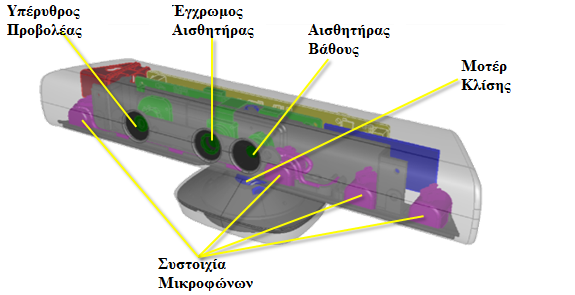
\includegraphics[width=.7\textwidth]{fig/kinect-characteristics.png}
    \caption{Δυνατότητες του αισθητήρα \eng{Kinect}\protect\footnotemark}
    \label{fig:kinect-characteristics}
\end{figure}
\footnotetext{Εικόνα από την ιστοσελίδα \eng{\url{http://msdn.microsoft.com/en-us/library/jj131033.aspx}}}

Ο αισθητήρας βάθους αποτελείται από ένα υπέρυθρο προβολέα λέιζερ σε συνδυασμό με ένα μονόχρωμο αισθητήρα \eng{CMOS}, ο οποίος καταγράφει δεδομένα βίντεο σε \eng{3D} κάτω από σχεδόν οποιεσδήποτε συνθήκες φωτισμού. Σύμφωνα με τις πληροφορίες που παρέχονται στους εμπόρους λιανικής πώλησης, το \eng{Kinect} είναι σε θέση να εντοπίζει ταυτόχρονα έως έξι άτομα. Ο χάρτης βάθους που δημιουργείται από τον αισθητήρα βάθους είναι στην ουσία μία εικόνα, η οποία χρησιμοποιώντας διαφορετικές αποχρώσεις χρώματος ανάλογα με την απόσταση τον αντικειμένων. Αν σκεφτεί κανείς το μικρό σχετικό κόστος με τις δυνατότητες και την πληροφορία που σου παρέχει το \eng{Kinect}, μπορούν να αναπτυχθούν πολύ ενδιαφέρουσες εφαρμογές \cite{jean13}. Στον πίνακα \ref{tab:sensor-characteristics} συνοψίζονται τα βασικά τεχνικά χαρακτηριστικά λειτουργίας.

\begin{center}
    \begin{tabular}{ll}
        \toprule
        % after \\: \hline or \cline{col1-col2} \cline{col3-col4} ...
        \multicolumn{2}{c}{Χαρακτηριστικά} \\
        \midrule
        Ανάλυση & $1280\times 960, \quad 1024\times 768,$ \\
          & $640\times 480, \quad 320\times 240$ \\
        Υπέρυθρη αόρατη δέσμη & $0.4m$ έως $3.5m$ \\
        Χάρτης βάθους, \eng{RGB} ροή δεδομένων & μέχρι 30 \eng{FPS} \\
        Ρύθμιση κάθετης κλίσης & $\pm 27^{o}$ \\
        Κάθετο πεδίο ορατότητας & $43.5^{ο}$ \\
        Οριζόντιο πεδίο ορατότητας & $57^{ο}$ \\
        \bottomrule
    \end{tabular}
    \captionof{table}{Χαρακτηριστικά του αισθητήρα \eng{Kinect}}
    \label{tab:sensor-characteristics}
\end{center}

\begin{figure}[H]
    \centering
    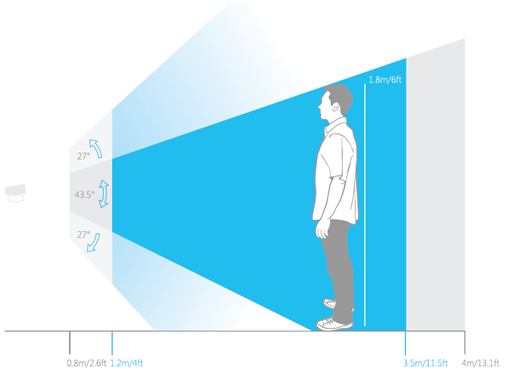
\includegraphics[width=.7\textwidth, height=.35\textheight]{fig/kinect-operation-mode.png}
    \caption{Περιγραφή περιοχών λειτουργίας\protect\footnotemark}
    \label{fig:kinect-operation-mode}
\end{figure}
\footnotetext{Εικόνα από την ιστοσελίδα \eng{\url{http://msdn.microsoft.com/en-us/library/hh973071.aspx}}}

%%%%%%%%%%%%%%%%%%%%%%%%%%%%%%%%%%%%%%%%%%%%%%%%%%%%%%%%%%%%%%%%%%%%%%%%%%%%%%%%
\subsection{Αλγόριθμος Ανίχνευσης Σκελετού}

Η υλοποίηση ενός αλγορίθμου ανίχνευσης του σκελετού είναι ένα δύσκολο κομμάτι που σχετίζεται με το κλάδο της υπολογιστικής όρασης \cite{mubarak97}, αλλά και άλλων κλάδων. Η ανίχνευση του σκελετού έχει μελετηθεί σε βάθος \cite{moseslund01, poppe07} στο παρελθόν. Με την δυνατότητα στερεοσκοπικής όρασης, αλλά και τον στόχο να αλληλεπιδρά με τον άνθρωπο η ομάδα έρευνας της \eng{Microsoft} υλοποιείται εσωτερικά έναν αλγόριθμο εκτίμησης της στάσης του ανθρώπου και την θέση των αρθρώσεων \cite{shotton11} με κριτήρια, τόσο στην ακρίβεια των αποτελεσμάτων, όσο και στην ταχύτητα για εφαρμογές πραγματικού χρόνο.

\begin{figure}[H]
    \centering
    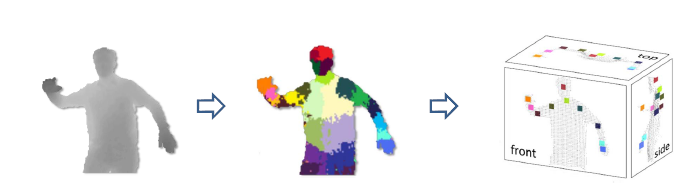
\includegraphics[width=.9\textwidth]{fig/kinect-skeleton-algorithm.png}
    \caption{Διαδικασία εξαγωγής των αρθρώσεων \cite{shotton11}}
    \label{fig:kinect-skeleton-algorithm}
\end{figure}
%\footnotetext{Εικόνα από την δημοσίευση \cite{shotton11}}

Υπάρχουν δύο υλοποιημένοι αλγόριθμοι ο \eng{body part classification} και ο \eng{offset joint regression}. Θα δώσουμε έμφαση στον πρώτο αλγόριθμο. Αρχικά χρησιμοποιώντας τον χάρτη βάθους για κάθε εικονοστοιχείο υπολογίζεται η συνάρτηση απόστασης \ref{equ:kinect-algorithm-feature-function} δίνοντας διαφορετικές τιμές στην $\phi$ ώστε να σαρώσει τον γύρο χώρο. Η συνάρτηση απόστασης μπορεί να υπολογιστεί εύκολα και παράλληλα για κάθε εικονοστοιχείο.

\begin{equation}
    f(u|\phi ) = z\big( u + \frac{\delta_1}{z(u)}\big)-z\big( u + \frac{\delta_2}{z(u)}\big)
    \label{equ:kinect-algorithm-feature-function}
\end{equation}

Όπου το $\phi = (\delta_1, \delta_2)$ είναι το χαρακτηριστικό που περιγράφει τις 2\eng{D} μετατοπίσεις από το εικονοστοιχείο \eng{u}, η $z(u)$ δίνει την τιμή βάθους του εικονοστοιχείου. Στην συνέχει χρησιμοποιώντας τυχαιοποιημένα δέντρα απόφασης (\eng{randomized decision forest}) γίνεται μια ταξινόμηση για τις συγκεκριμένες παραμέτρους $\phi$ και εκτιμάται μια πυκνότητα πιθανότητας, που υποδηλώνει σε ποιο τμήμα του σώματος ανήκει το εικονοστοιχείο. Η διαδικασία επαναλαμβάνεται για όλα τα δέντρα που ανήκουν στον σύνολο και για κάθε εικονοστοιχείο. Τέλος υπολογίζεται ο μέσος όρος για τον συγκεκριμένο εικονοστοιχείο από όλες τις πυκνότητες πιθανότητες που υπολογίστηκαν από κάθε δέντρο απόφασης τους συνόλου και ταξινομείται σε ένα τμήμα του σώματος.

\begin{equation}
    p(c|u) = \frac{1}{T} \cdot \sum_{l \in L(u)} p_{l}(c)
    \label{equ:kinect-algorithm-pixel-probability}
\end{equation}

Ως τελικό βήμα με βάση την ταξινόμηση των εικονοστοιχείων του χάρτη βάθους υπολογίζεται η τρισδιάστατη θέση των αρθρώσεων για κάθε τμήμα του σώματος και γίνεται παλινδρόμηση ενός γενικού μοντέλου (σκελετός). Κάτι που δεν αναφέρθηκε είναι ο τρόπος με τον οποίον επιλέγονται οι τιμές $\phi$, που ουσιαστικά είναι μια δειγματοληψία στην γειτονία του εικονοστοιχείου. Επίσης είναι φανερό ότι πρέπει να γίνει μια διαδικασία εκπαίδευσης του αλγορίθμου. Για να γίνει αυτό αρχικά συλλέχθηκαν εικόνες βάθους για τις οποίες ήταν ήδη γνωστή η θέση των αρθρώσεων και τα εικονοστοιχεία ήταν είδη ταξινομημένα στα αντίστοιχα τμήματα του σώματος. Στην συνέχει συνθέθηκαν κατάλληλα, επιπλέον εικόνες βάθους \ref{fig:kinect-data-synthesis} από τις υπάρχουσες με διαφορετικά ανθρωπομετρικά χαρακτηριστικά και με διαφορετικούς προσανατολισμούς της κάμερας ώστε να κάνουν τον αλγόριθμο πιο αξιόπιστο και γενικό.

\begin{figure}[H]
    \centering
    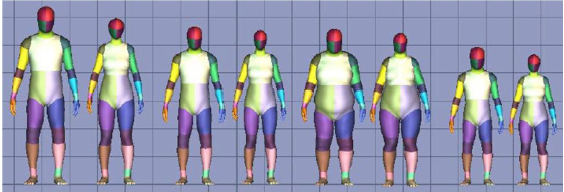
\includegraphics[width=.9\textwidth]{fig/kinect-data-synthesis.png}
    \caption{Συνθέσεις των εικόνων βάθους για την εκπαίδευση του αλγορίθμου \cite{shotton11}}
    \label{fig:kinect-data-synthesis}
\end{figure}
%\footnotetext{Εικόνα από την δημοσίευση \cite{shotton11}}

Το πρόβλημα είναι πολύ δύσκολο και εξαρτάται από πολλούς παράγοντες, όπως είναι το φως, η διαφοροποίηση των ανθρώπων, οι ποικίλες στάσεις, το χρώμα, το δίσημο και από παρεμπόδιση τμημάτων του σώματος που δεν είναι ορατά στον αισθητήρα (\eng{occlusion}). Ο αλγόριθμος επιτυγχάνει πολύ υψηλά ποσοστά ανίχνευσης με μεγάλη ακρίβεια. Είναι ταχύτατος, γιατί από την φύση του μπορεί να εκτελεστεί παράλληλα, με αποτέλεσμα η υλοποίηση του να γίνει στο υλικό εσωτερικά και όχι από λογισμικό.

%%%%%%%%%%%%%%%%%%%%%%%%%%%%%%%%%%%%%%%%%%%%%%%%%%%%%%%%%%%%%%%%%%%%%%%%%%%%%%%%
\section{Εργαλεία}

Υπάρχουν πολλές εναλλακτικές λύσεις για το ποιο εργαλείο μπορεί να χρησιμοποιηθεί για πρόσβαση στα δεδομένα που σου παρέχει το \eng{Kinect}. Παρακάτω θα αναφερθούν δύο εργαλεία: το προκαθορισμένο \eng{SDK} της \eng{Microsoft} και το εναλλακτικό της \eng{OpenNI}. Και τα δύο είναι εξίσου καλά και χρησιμοποιούνται από πολλούς χρήστες. Τα εργαλεία σου παρέχουν επιπλέον δυνατότητες για πιο προχωρημένες εφαρμογές όπως είναι η αναγνώριση ομιλίας, αναγνώριση έκφρασης προσώπου, τρισδιάστατη ανακατασκευή και πολλά άλλα. Παρακάτω αναφέρονται κάποια βασικά χαρακτηριστικά των δύο εγαλείων.

%%%%%%%%%%%%%%%%%%%%%%%%%%%%%%%%%%%%%%%%%%%%%%%%%%%%%%%%%%%%%%%%%%%%%%%%%%%%%%%%
\subsection{\texorpdfstring{Προκαθορισμένο Εργαλείο της \eng{Microsoft}}{}}

Το εργαλείο της \eng{Microsoft} είναι δωρεάν και παρέχει πλούσιο ρεπερτόριο από συναρτήσεις για πρόσβαση στην συσκευή. Είναι αποκλειστικά για \eng{Windows} και δεν μπορεί να χρησιμοποιηθεί από αλλά λειτουργικά. Οι γλώσσες προγραμματισμού που χρησιμοποιούνται είναι η \eng{C++} και η \eng{C\#}. Υπάρχει δυνατότητα συνεργασία με άλλες βιβλιοθήκες, όπως είναι η \eng{XNA} και το \eng{DirectX}.

Όσον αφορά την απόκτηση σκελετικής πληροφορίας υπάρχει μια μεγάλη διαφορά στο ότι το \eng{SDK} της \eng{Microsoft} σου παρέχει πληροφορία 20 αρθρώσεων. Ένα σημαντικό πλεονέκτημα σε σχέση με άλλα εργαλεία είναι ότι δεν απαιτείται βαθμονόμιση του αισθητήρα. Επίσης μπορεί κανείς να ανιχνεύει μέχρι έξι σκελετούς στην εφαρμογή του. Τέλος, σου παρέχει έτοιμες δομές φίλτρων για την βελτίωση του αποτελέσματος της ακολουθίας των θέσεων, που είναι μια απαραίτητη διαδικασία αφού υπάρχει πάντα θόρυβος και προβλήματα εκτίμησης της θέσης. Στην εικόνα \ref{fig:microsoft-sdk-skeleton} φαίνεται ενδεικτικά η δομή του σκελετού που σου προσφέρει το συγκεκριμένο εργαλείο.

\begin{figure}[H]
    \centering
    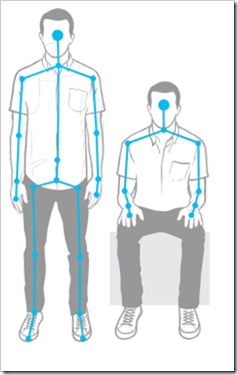
\includegraphics[height=.35\textheight]{fig/microsoft-skeleton.png}
    \caption{Σκελετικό σύστημα που παρέχει το εργαλείο της \eng{Microsoft}\protect\footnotemark}
    \label{fig:microsoft-sdk-skeleton}
\end{figure}
\footnotetext{Εικόνα από την ιστοσελίδα \eng{\url{http://msdn.microsoft.com/en-us/library/hh973077.aspx}}}

%%%%%%%%%%%%%%%%%%%%%%%%%%%%%%%%%%%%%%%%%%%%%%%%%%%%%%%%%%%%%%%%%%%%%%%%%%%%%%%%
\subsection{\texorpdfstring{Εναλλακτικό Εργαλείο της \eng{OpenNI}}{}}

Το εναλλακτικό εργαλείο είναι το \eng{OpenNI} εκτός από το \eng{Kinect} δίνει την δυνατότητα πρόσβασης και σε άλλους αισθητήρες με τον ίδιο τρόπο και έχει μια ξεκάθαρη αρχιτεκτονική, που διευκολύνει τον προγραμματιστή όπως φαίνεται στην εικόνα \ref{fig:openni-framework}. Όμοια με το \eng{SDK} της \eng{Microsoft} η \eng{OpenNI} σου παρέχει πλούσιο ρεπερτόριο από αλγορίθμους και εφαρμογές. Είναι ανοιχτού κώδικα, υπάρχει υλοποίηση όσο στα \eng{Windows}, έτσι και στο \eng{Linux} (\eng{cross platform}). Οι κύριες γλώσσες προγραμματισμού  που υποστηρίζονται από το \eng{OpenNI} είναι η \eng{C++}, η \eng{Java} και \eng{Python}.

\begin{figure}[H]
    \centering
    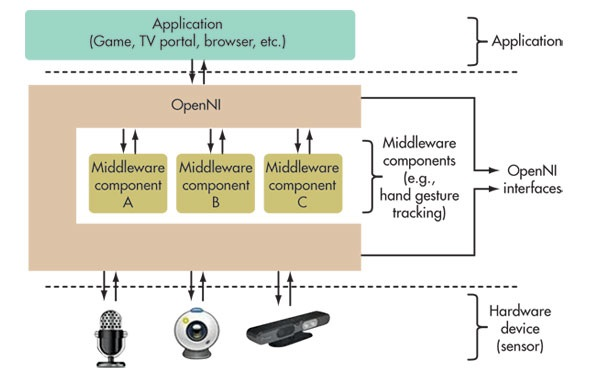
\includegraphics[width=.7\textwidth, height=.3\textheight]{fig/openni-framework.jpg}
    \caption{Αρχιτεκτονική της βιβλιοθήκης της \eng{OpenNI}\protect\footnotemark}
    \label{fig:openni-framework}
\end{figure}
\footnotetext{Εικόνα από την ιστοσελίδα \eng{\url{http://electronicdesign.com/embedded/how-microsoft-s-primesense-based-kinect-really-works}}}

\begin{figure}[H]
    \centering
    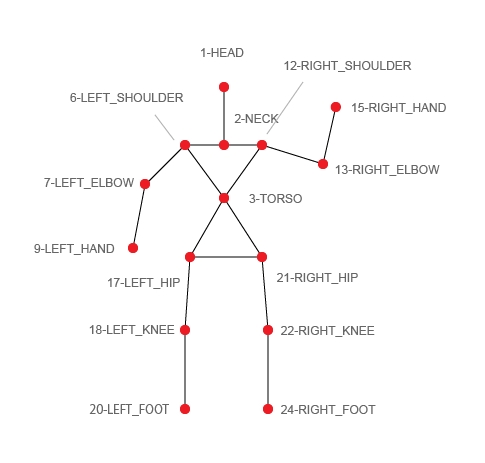
\includegraphics[width=.5\textwidth]{fig/openni-skeleton.png}
    \caption{Σκελετικό σύστημα που προσφέρει το εργαλείο της \eng{OpenNI}}
    \label{fig:openni-skeleton}
\end{figure}

Όσον αφορά την εξαγωγή του σκελετού, μειονεκτεί σε σύγκριση με τον αντίστοιχο εργαλείο της \eng{Microsoft}. Αυτό γιατί σου παρέχει 16 αρθρώσεις όπως φαίνεται στην εικόνα \ref{fig:openni-skeleton}, που ίσως δεν είναι αρκετά για την εφαρμογή, ειδάλλως δεν είναι και τόσο κρίσιμη διαφορά. Ένα βασικό μειονέκτημα είναι η απαίτηση βαθμονόμησης της συσκευής. Επίσης κάτι σημαντικό είναι το κομμάτι που αφορά την βελτίωση των μετρήσεων και το \eng{OpenNI} δεν σου παρέχει έτοιμες δομές, κάτι που θα χρειαστεί χρόνο για να υλοποιηθεί. Για τους παραπάνω λόγους προτιμήθηκε το εργαλείο της \eng{Microsoft}. Ενδεικτικά στον πίνακα \ref{tab:openni-microsoft} φαίνονται κάποιες βασικές διαφορές.

\begin{center}
    \begin{tabular}{lcc}
        \toprule
        % after \\: \hline or \cline{col1-col2} \cline{col3-col4} ...
        \multicolumn{1}{c}{Χαρακτηριστικά} & \eng{OpenNI} & \eng{Microsoft SDK} \\
        \midrule
        Πρόσβαση στα δεδομένα βάθους και \eng{RGB} & Ναι & Ναι \\
        Ανίχνευση αρθρώσεων & Ναι & Ναι \\
        Υποστήριξη αναγνώρισης χειρονομιών & Ναι & Όχι \\
        Συναρτήσεις άμεσης αποθήκευσης δεδομένων στο δίσκο & Ναι & Όχι \\
        Βαθμονόμιση & Ναι & Όχι \\
        Υποστήριξη επεξεργασίας ήχου και αναγνώριση ομιλίας & Όχι & Ναι \\
        Ευκολία εγκατάστασης & Όχι & Ναι \\
        Διαθέσιμος αριθμός αρθρώσεων & 16 & 20 \\
        Ποιότητα εγχειριδίων τεκμηρίωσης  & Καλή & Μέτρια\\
        \bottomrule
    \end{tabular}
    \captionof{table}{Σύγκριση βασικών χαρακτηριστικών μεταξύ των δύο εργαλείων}
    \label{tab:openni-microsoft}
\end{center}

%%%%%%%%%%%%%%%%%%%%%%%%%%%%%%%%%%%%%%%%%%%%%%%%%%%%%%%%%%%%%%%%%%%%%%%%%%%%%%%%
\section{Σύστημα Μετρήσεων}

Η συλλογή ορθών μετρήσεων είναι ένα σημαντικό βήμα για την εξαγωγή σωστών αποτελεσμάτων στα μετέπειτα στάδια. Η καταγραφή της βάδισης του ανθρώπου είναι η βάση για πολλές αναλύσεις, όπου μπορούν να εξαχθούν χρήσιμα αποτελέσματα. Ενδεικτικά θα ήταν χρήσιμη η μελέτη της δυναμικής συμπεριφοράς του σώματος κατά την διεξαγωγή μιας κίνησης, με αποτέλεσμα να μπορεί κανείς να μελετήσει την συμπεριφορά του μυοσκελετικού συστήματος. Πρέπει να δοθεί μεγάλη βαρύτητα στην απόκτηση έγκυρων μετρήσεων, για το λόγο αυτό απαιτείται η δημιουργία αλγορίθμων που θα ελαχιστοποιούν τα σφάλματα και θα διώχνουν τον θόρυβο. Στην συνέχεια εξηγούμε κάποια ενδεικτικά προβλήματα κατά την διαδικασία της καταγραφής και την αντιμετώπιση τους.

%%%%%%%%%%%%%%%%%%%%%%%%%%%%%%%%%%%%%%%%%%%%%%%%%%%%%%%%%%%%%%%%%%%%%%%%%%%%%%%%
\subsection{Τροχιές των Αρθρώσεων}

Ο προγραμματιστής  μπορεί να έχει πρόσβαση στα δεδομένα της συσκευής που αφορούν την συντεταγμένη των αρθρώσεων. Δεδομένου ότι έχει ενεργοποιηθεί εσωτερικά (από τον πρόγραμμα) η ανίχνευση του σκελετού και στο πεδίο ορατότητας της συσκευής ανιχνευθεί αντικείμενο ανθρώπινης μορφής, τότε η συσκευή στέλνει πακέτα με την πληροφορία των θέσεων των αρθρώσεων πίσω στον χρήστη. Το πακέτο περιέχει και επιπλέον πληροφορίες για τις αρθρώσεις όπως είναι ο προσανατολισμός (προϋποθέτει ιεραρχική δομή σκελετού), σκορ εμπιστοσύνης για την μέτρηση (που κυμαίνεται από 0 έως 1) και κάποιες ενδείξεις αν έχει εξαχθεί συμπέρασμα για την θέση της άρθρωσης. Στην ανάλυση ενδιαφερόμαστε για την θέση όσο εξελίσσεται ο χρόνος. Έστω ότι έχουμε $Ν$ αριθμό αρθρώσεων που αποθηκεύονται σε συγκεκριμένες χρονικές στιγμές.

\begin{equation}
    p^{t}_{j} = \{x^{t}_{j}, y^{t}_{j}, z^{t}_{j}\}, \quad t \in (0, t), \quad j \in (0, N)
    \label{equ:trajectories}
\end{equation}

Όπου \eng{p} είναι η Καρτεσιανή θέση την χρονική στιγμή \eng{t} για την άρθρωση \eng{j}. Η αρχή των αξόνων είναι η θέση του \eng{Kinect} και ο άξονας \eng{Z} είναι το βάθος όπως φαίνεται στην εικόνα \ref{fig:kinect-joints}.

\begin{figure}[H]
    \centering
    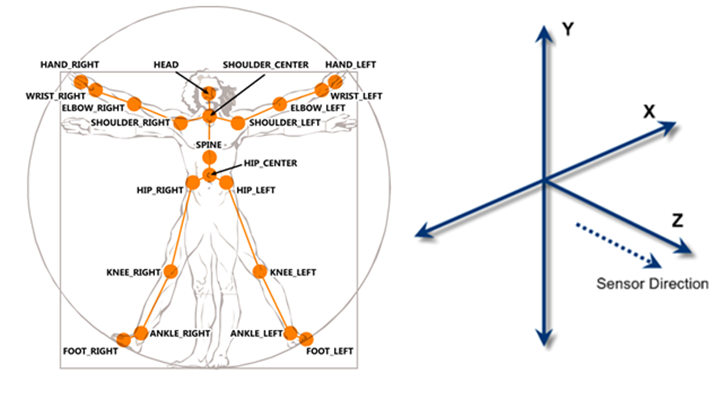
\includegraphics[width=.8\textwidth]{fig/kinect-joints.png}
    \caption{Το σύστημα αρθρώσεων που χρησιμοποιήθικαι\protect\footnotemark}
    \label{fig:kinect-joints}
\end{figure}
\footnotetext{Εικόνα από την ιστοσελίδα \eng{\url{http://msdn.microsoft.com/en-us/library/jj131025.aspx}}}

Πρέπει να διευκρινιστεί ότι τα δεδομένα δεν έρχονται περιοδικά σε ντετερμινιστικές χρονικές στιγμές, αλλά έχουν μια απόκλιση που οφείλεται κυρίως στο \eng{software} και στις εσωτερικές καθυστερήσεις. Για το λόγο αυτό είναι χρήσιμο να γίνει η μέτρηση της χρονικής στιγμής που έρχονται και αποθηκεύονται τα δεδομένα ώστε να χρησιμοποιηθεί στα μετέπειτα στάδια της ανάλυσης. Μια άλλη παρατήρηση είναι ότι τα δεδομένα βρίσκονται στο σύστημα συντεταγμένων με αρχή των αξόνων το \eng{Kinect} και ανάλογα το εργαλείο που θα χρησιμοποιηθεί στα μετέπειτα στάδια της επεξεργασίας θα πρέπει να γίνει η κατάλληλη μετατροπή συστήματος συντεταγμένων.

%%%%%%%%%%%%%%%%%%%%%%%%%%%%%%%%%%%%%%%%%%%%%%%%%%%%%%%%%%%%%%%%%%%%%%%%%%%%%%%%
\subsection{Αντιμετώπιση του Θορύβου}

Υπάρχουν πολλά ενοχλητικά προβλήματα που εμφανίζονται στην πράξη και καθιστούν τις μετρήσεις \lq μην κατάλληλες\rq\: για επεξεργασία. Ο θόρυβος επηρεάζεται από πολλούς παράγοντες, όπως είναι ο φωτισμός στον χώρο που διεξάγεται το πείραμα, η στάση του σώματος, η τοποθεσία της συσκευής και πολλά άλλα. Ένα πολύ εμφανές παράδειγμα θορύβου που εμφανίζεται κατά την εκτίμηση της θέσης της άρθρωσης, λόγω της μικρής απόκλιση της τιμής από την προηγούμενη μέτρηση, με αποτέλεσμα να δίνει την αίσθηση ότι το δείγμα τρέμει, ενώ στην πραγματικότητα είναι στάσιμο όπως φαίνεται και στην εικόνα \ref{fig:hand2}.

\begin{figure}[h]
    \centering
    \begin{subfigure}[b]{.4\textwidth}
        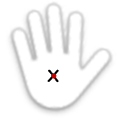
\includegraphics[width=\textwidth]{fig/hand1.png}
        \caption{Βέλτιστη εκτίμηση της θέσης του χεριού}
        \label{fig:hand1}
    \end{subfigure} ~
    \begin{subfigure}[b]{.4\textwidth}
        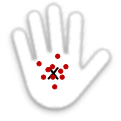
\includegraphics[width=\textwidth]{fig/hand2.png}
        \caption{Εκτίμηση της θέσης του χεριού λόγω θορύβου}
        \label{fig:hand2}
    \end{subfigure}
    \caption{Πρόβλημα εκτίμησης θέσης λόγω θορύβου\protect\footnotemark}
\end{figure}
\footnotetext{Εικόνα από την ιστοσελίδα \eng{\url{http://msdn.microsoft.com/en-us/library/jj131429.aspx}}}

Για την αντιμετώπιση του προβλήματος μπορούν να υλοποιηθούν απλές τεχνικές φιλτραρίσματος και να ελαχιστοποιηθεί ο θόρυβος. Πρέπει κανείς να ξεχωρίσει κάποια κριτήρια που είναι το ποσοστό της εξομάλυνσης των πολύ απότομων κινήσεων, την καθυστέρηση που εισάγεται από την αλλαγή που προκαλεί η φάση του φίλτρου και το αν η εφαρμογή είναι πραγματικού χρόνου (\eng{online}) ή μην πραγματικού χρόνου (\eng{offline}).

Αν επιλεχθεί να αποκοπούν οι ψηλές συχνότητες (απότομες κινήσεις), τότε θα αντιμετωπιστεί το πρόβλημα που αναφέρθηκε πιο πάνω και το αποτέλεσμα θα είναι αυτό της εικόνας \ref{fig:hand1}. Ο θόρυβος αυτής της μορφής στην ξένη βιβλιογραφία αναφέρεται σαν \lq \eng{jitter}\rq . Πρέπει να προσέξουμε όμως, γιατί το σύστημα θα αγνοεί πέραν του θορύβου και τις απότομες κινήσεις του δείγματος που ίσως είναι κάτι ανεπιθύμητο. Η σωστή επιλογή αυτών των παραμέτρων είναι κρίσιμη και εξαρτάται από την εφαρμογή που μας ενδιαφέρει και κυρίως από την ταχύτητα του δείγματος.

Όπως φαίνεται στην εικόνα \ref{fig:filter-latency} με κόκκινο είναι η τροχιά, όπου βλέπουμε τις ανεπιθύμητες μεταβολές λόγω θορύβου. Από την άλλη με μπλε χρώμα είναι η τροχιά μετά το φιλτράρισμα, όπου παρατηρούμε ότι έχει εξομαλυνθεί ο θόρυβος, αλλά έχει δημιουργηθεί καθυστέρηση των δειγμάτων. Κάτι που αξίζει να σημειωθεί είναι ότι αν η εφαρμογή δεν απαιτείται να είναι πραγματικού χρόνου, τότε μπορούν να χρησιμοποιηθούν μην αιτιατά φίλτρα, που λαμβάνουν υπόψη στους υπολογισμούς τις μελλοντικές τιμές, με αποτέλεσμα να γίνει καλύτερη εκτίμηση της τροχιάς.

\begin{figure}[h]
    \centering
    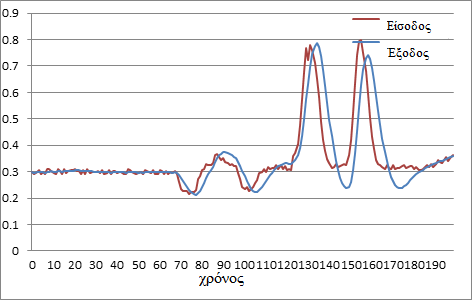
\includegraphics[width=.8\textwidth]{fig/filter-latency.png}
    \caption{Εξομάλυνση και καθυστέρηση της ακολουθίας μετά το φιλτράρισμα\protect\footnotemark}
    \label{fig:filter-latency}
\end{figure}
\footnotetext{Εικόνα από την ιστοσελίδα \eng{\url{http://msdn.microsoft.com/en-us/library/jj131429.aspx}}}

Για παράδειγμα μια απλή τεχνική για την αφαίρεση του θορύβου λόγω \eng{jitter} βασίζεται στην απλή σχέση αναδρομής \ref{equ:jitter-removal}.

\begin{equation}
    \hat{p}_{n} =
    \begin{cases}
        p_{n}, & \text{Αν } \|p_{n} - \hat{p}_{n-1}\| < \text{κατώφλι} \\
        a \cdot p_{n} + (1-a) \cdot \hat{p}_{n-1}, & \text{αλλιώς}
    \end{cases}
    \label{equ:jitter-removal}
\end{equation}

Στην παρούσα εργασία χρησιμοποιείται μια παραλλαγή του φίλτρου \cite{filter12} \lq \eng{Holt Double Exponential Smoothing}\rq , που έχει άμεση εφαρμογή στα οικονομικά. Τα φίλτρα αυτά στηρίζονται στην παρακάτω αναδρομική σχέση \ref{equ:double-exponential} και οι παράμετροι που επηρεάζουν το αποτέλεσμα δίνονται στο πίνακα \ref{tab:filter-parameters}.

\begin{equation}
    \begin{aligned}
        b_{n} = \gamma \cdot (\hat{p}_{n} - \hat{p}_{n-1}) + (1 - \gamma) \cdot b_{n-1}\\[10pt]
        \hat{p}_{n} = \alpha \cdot p_{n} + (1 - a) \cdot (\hat{p}_{n-1} + b_{n-1})
    \end{aligned}
    \label{equ:double-exponential}
\end{equation}

\vspace{10pt}

\begin{center}
    \begin{threeparttable}
        \begin{tabular}{lccc}
            \toprule
            % after \\: \hline or \cline{col1-col2} \cline{col3-col4} ...
            Παράμετροι & Κανονικό\tnote{α} & Μέτριο\tnote{β} & Δυνατό\tnote{γ} \\
            \midrule
            \eng{Smoothing} & 0.5 & 0.5 & 0.7 \\
            \eng{Correction} & 0.5 & 0.1 & 0.3 \\
            \eng{Prediction} & 0.5 & 0.5 & 1.0 \\
            \eng{JitterRadius} & 0.05 & 0.1 & 1.0 \\
            \eng{MaxDeviationRadius} & 0.04 & 0.1 & 1.0 \\
            \bottomrule
        \end{tabular}
        \begin{tablenotes}
            \item[α] Φιλτράρει ελαφρώς το \eng{jitter}. Καλό για εφαρμογές αναγνώρισης σε παιχνίδια, όπου υπάρχουν απότομες κινήσεις.
            \item[β] Μειώνει αρκετά το \eng{jitter}. Είναι καλό για εφαρμογές όπου απαιτείται ομαλή κίνηση.
            \item[γ] Μειώνει πολύ το \eng{jitter}. Αφορά εφαρμογές που δεν ενδιαφερόμαστε για την καθυστέρηση της κίνησης.
        \end{tablenotes}
    \end{threeparttable}
    \captionof{table}{Ενδεικτικοί παράμετροι του φίλτρου}
    \label{tab:filter-parameters}
\end{center}

%\begin{itemize}
%	\item \eng{Smoothing} παράμετρος εξομάλυνσης
%	\item \eng{Correction} μικρές τιμές τείνουν να μοιάζουν με τα δεδομένα που έχουμε
%	\item \eng{Prediction} συμβολίζει την εκτίμηση που κάνουμε για μελλοντικές τιμές
%	\item \eng{JitterRadius} η ακτίνα σε μέτρα για την μείωση του \eng{jitter}
%    \item \eng{MaxDeviationRadius} η μέγιστη διασπορά στην ακτίνα την οποία μπορεί να ανεχτεί το φίλτρο
%\end{itemize}

